\begin{figure}
\newcommand{\wsd}{\columnwidth+1.3cm}  % width solar decomp
\newcommand{\hsd}{4cm}  % height solar decomp
\newcommand{\srd}{../figures/decomposition/11-Feb-02-solar-s}  % solar decomp results dir
\newcommand{\mbs}{\hspace{-0.8cm}}  % move back
\begin{tabular}{c}
\mbs 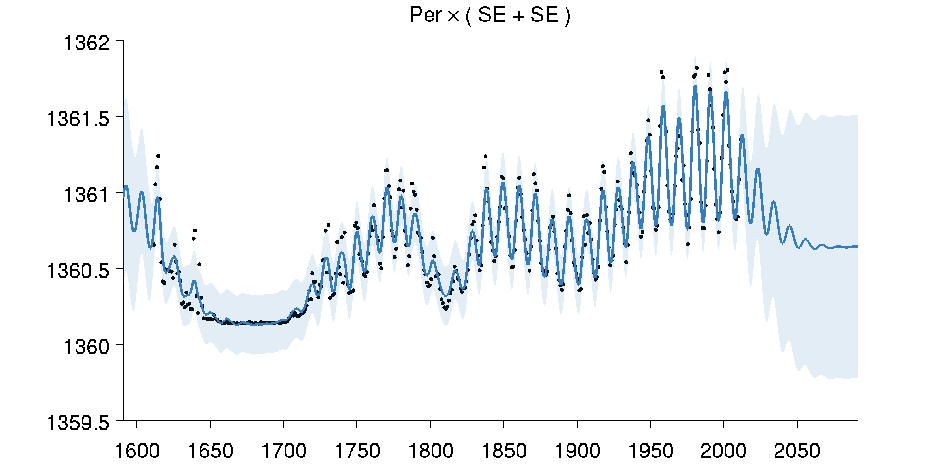
\includegraphics[width=\wsd,height=\hsd]{\srd/02-solar-s_all} \\
\mbs 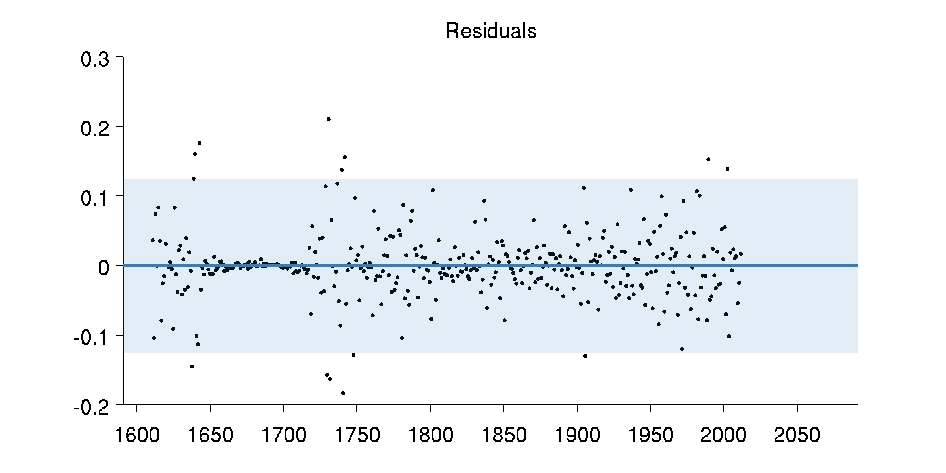
\includegraphics[width=\wsd,height=\hsd]{\srd/02-solar-s_resid}
\end{tabular}
\caption{Full posterior and residuals on the solar irradiance dataset.}
\label{fig:solar_decomp}
\end{figure}
